%%%%%%%%%%%%%%%%%%%%%%%%%%%%%%%%%%%%%%%%%%%%%%%%%%%%%%%%%%%%%%%%%%% 
%                       rpithes-short.tex                         %
%         Template for a short thesis all in one file             %
%        (titlepage info below assumes masters degree}            %
%  Just run latex (or pdflatex) on this file to see how it looks  %
%      Be sure to run twice to get correct TOC and citations      %
%%%%%%%%%%%%%%%%%%%%%%%%%%%%%%%%%%%%%%%%%%%%%%%%%%%%%%%%%%%%%%%%%%% 
%
%  To produce the abstract title page followed by the abstract,
%  see the template file, "abstitle-mas.tex"
%
%%%%%%%%%%%%%%%%%%%%%%%%%%%%%%%%%%%%%%%%%%%%%%%%%%%%%%%%%%%%%%%%%%%

\documentclass{thesis}
\usepackage{graphicx}
\usepackage{url}
\usepackage{subfig}

% Use the first command below if you want captions over 1 line indented.
% A side effect of this is to remove the use of bold for captions. 
% To restore bold, also include the second line below.
%\usepackage[hang]{caption}     % to indent subsequent lines of captions
\renewcommand{\captionfont}{\bfseries} % only needed with caption package;
                                        %   otherwise bold is default)
\renewcommand{\topfraction}{0.99}
\renewcommand{\bottomfraction}{0.99}
\renewcommand{\textfraction}{0.01}
\renewcommand{\floatpagefraction}{0.01}
\renewcommand{\dbltopfraction}{0.99}
\renewcommand{\dblfloatpagefraction}{0.01}
%%%%%%%%%%%%%%%%%%%%  supply titlepage info  %%%%%%%%%%%%%%%%%%%%%
\thesistitle{\bf Thin Shell Structure Design Tool}        
\author{R. Allan Pendergrast}
\degree{Master of Science}
\department{Computer Science}
\thadviser{Barbara M. Cutler}
\submitdate{May 2010\\(For Graduation May 2010)}        
%\copyrightyear{1685}  % if date omitted, current year is used. 
%%%%%%%%%%%%%%%%%%%%%   end titlepage info  %%%%%%%%%%%%%%%%%%%%%%
      
\begin{document} 
\titlepage             % Print titlepage   
%\copyrightpage        % optional         
\tableofcontents       % required 
\listoftables          % required if there are tables
\listoffigures         % required if there are figures

\specialhead{ACKNOWLEDGMENT}
Thanks to Barbara Cutler for all her help in creating, testing, and writing about this tool.

\specialhead{ABSTRACT}
Thin-shell structures are becoming increasingly useful in construction and design of buildings.  They allow the usage of less material to enclose
larger spaces, are structurally efficient, and have a natural aesthetic beauty.  However, they can be difficult to design, as the exact shape
required for structural stability depends on the material used, the size of the shell, and other features.  Fortunately, it is possible to simulate
these structures quickly and accurately, allowing architects to concentrate more on their design and less on ensuring that their building is
stable.  The tool described in this thesis simulates thin-shell structures and aids architects in their design and optimization.

\chapter{INTRODUCTION} \label{chp:introduction}

\section{Project Goals} \label{sec:goals}
The goal of this project was to create a tool that could be used by architects to construct buildings more cheaply.  There are many factors
that can make construction of a building expensive.  Labor, materials, and planning are all expensive elements which can be optimized.
This project focuses primarily on the third of these, reducing design time by giving the architect a tool that allows them to quickly design a
structurally efficient building.

Structural efficiency is a very important element of construction.  With traditional construction methods, this tends not to be an issue, since
the tried-and-true construction conventions will keep a building standing.  Houses, for example, have been built using the same structural
conventions for years and do not require any advanced structural analysis.  Walls are constructed with studs every 16 inches, and the house
stands up.  Even in non-residential structures, the studded or cinder-block walls convention tends to be followed.  However, when creating
buildings that fall outside the norm of studded walls, cinder block construction, and other such traditional methods, more complex analysis
tools are necessary.  Insufficient analysis of the elements used in constructing a building can result in spectacular disasters such as those
detailed and discussed in \underline{Why Buildings Fall Down}\cite{levy92falldown}.  Conversely, if proper care is taken to analyze structures
before they are constructed, miracles of architecture can be constructed that stand up for thousands of years, as some of the building in
Mario Salvadori's \underline{Why Buildings Fall Down}\cite{salvadori80standup} have.

%This project was originally conceived as a structural analysis tool that would find highly over- or underloaded members in a structure
%and notify the architect that some force could be diverted towards the less-used member or that the underloaded member could be
%removed.  This redesigning would help to optimize the structure, resulting in a structure that required less material or work to construct.
%Since then, the focus has shifted to the design and optimization of thin shell structures.  These structures, covered in more detail in
%\ref{thinshell}, are used in architecture to conserve materials, funds, or for simply aesthetic reasons.  Unfortunately, thin-shell
%structures have been famously difficult to optimize and construct, sometime requiring a complete overhaul of the structure to fix stability
%problems. This tool attempts to alleviate this difficulty and make the design and optimization of such structures easier and faster for architects.

\section{Thin Shell Structures} \label{thinshell}

\subsection{Overview}
A thin shell structure is a structure which has a small thickness compared to its other dimensions.  While this may seem to be
an obvious definition, the design and construction of these structures can be complicated.  In traditional construction, load-bearing
members are flat, carrying forces straight through themselves.  A simplified 2D representation of the load-bearing elements of a house
can be seen in Figure \ref{fig:house}.  Larger buildings which are constructed using traditional techniques use very similar techniques
as those used in Figure \ref{fig:house}, employing vertical members and cross-pieces to support the weight of the building.  One
consideration for larger buildings is that large rooms will have large unsupported expanses of floor.  Beams which are loaded transversely
in that manner are subjected to bending according to the Euler-Bernoulli equation: \[EI\frac{d^4u}{dx^4}=w(x)\]
If too much force is applied, the beam will buckle, perhaps causing catastrophic failure.  Therefore, beams and other flat structural
elements must have a high second moment of area (have a large dimension parallel to the applied force) in order to ensure that it will not
buckle under load.  Alternately, columns can be installed to effectively shorten the span which the beam is crossing, but depending on the
application, this may not be desirable.

\begin{figure}
\centering
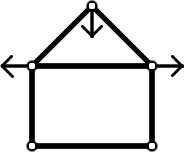
\includegraphics[width=2in]{images/house.png}
\caption[Simplified representation of a house]{This simplified representation of the load-bearing elements of a house show how traditional
construction techniques require additional material to be stable.  Were it not for the horizontal piece which forms the ceiling, the walls
would be forced outward by the forces caused by the weight of the roof.}
\label{fig:house}
\end{figure}

\begin{figure}
\centering
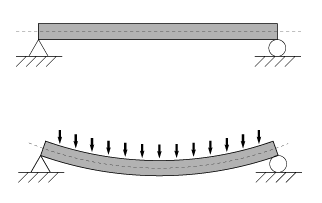
\includegraphics[width=4in]{images/Bending.png}
\caption[A beam under uniform loading]{This is an image of a beam which is deforming under a uniform load.  ``Bending", image created by Daniel De
Leon Martinez, \url+http://en.wikipedia.org/wiki/File:Bending.png+}
\label{fig:bending}
\end{figure}

Unlike normal beam and plate structures, thin shell structures are curved, which allows the force to travel through the thinner structural
elements.  Structures such as those in figure \ref{fig:isler_service} can cover a large span with a minimal amount of material, saving the
construction company money.  Since the structure completely supports itself, no internal columns are necessary, allowing an unobstructed interior.
An unobstructed interior is very useful in a variety of buildings such as theatres, museums, and airport terminals, to name a few.
These structures are very stable because of their unique shape, called a catenary shell.  Catenaries are covered in more detail in section
\ref{sec:catenary}  Some prominent thin shell structures include
the TWA Flight Center Building at the JFK International Airport in New York, New York (Fig. \ref{fig:twa_flight}), the Kresge Auditorium on
the MIT campus in Cambridge, Massachusetts (Fig. \ref{fig:kresge_aud}), and the Montreal Biosphere in Montreal, Canada (Fig \ref{fig:montreal_bio}).

\begin{figure}
\centering
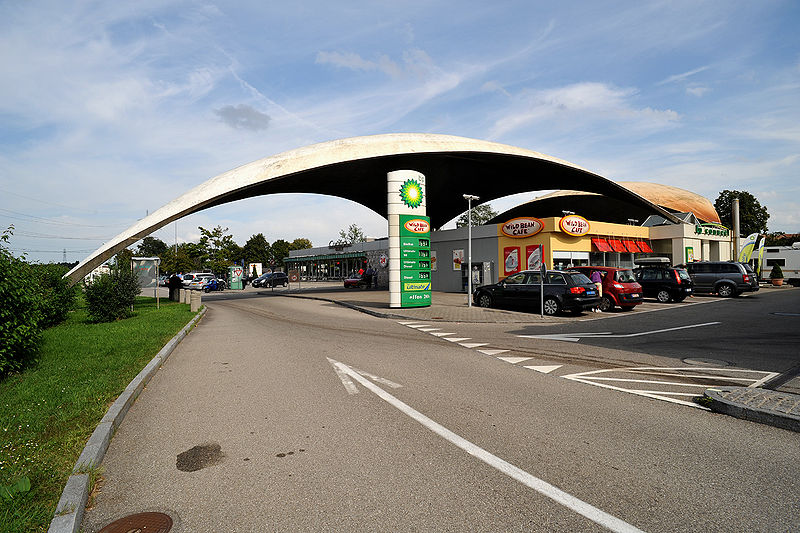
\includegraphics[width=4in]{images/isler_dome_1.jpg}
\caption[A thin-shell dome over a service area in Switzerland]{This dome, designed by Swiss civil engineer Heinz Isler, gracefully arches over
a service station along the A1 Motorway in Switzerland, protecting it from the elements with a minimal amount of material.  ``Deitingen Service
Station"(1968), Heinz Isler, photo taken by Chriusha, \url+http://commons.wikimedia.org/wiki/File:Deitingen_Sued_Raststaette,_Schalendach_04_09.jpg+}
\label{fig:isler_service}
\end{figure}

\begin{figure}
\centering
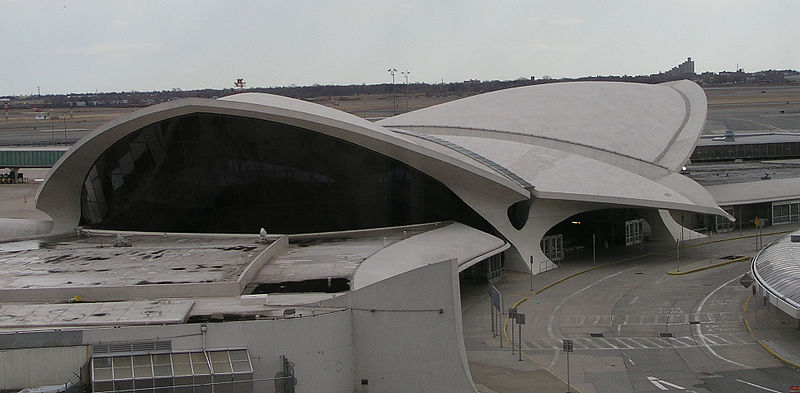
\includegraphics[width=5in]{images/twa_flight_center.jpg}
\caption[The TWA Flight Center]{The TWA Flight Center at JFK International Airport in New York, New York is an excellent modern example of
thin-shell structures providing a much-needed unobstructed internal space.  ``TWA Flight Center", Eero Saarinen, photo taken by Marc N. Weissman
\url+http://en.wikipedia.org/wiki/File:08terminal5.jpg+}
\label{fig:twa_flight}
\end{figure}

\begin{figure}
\centering
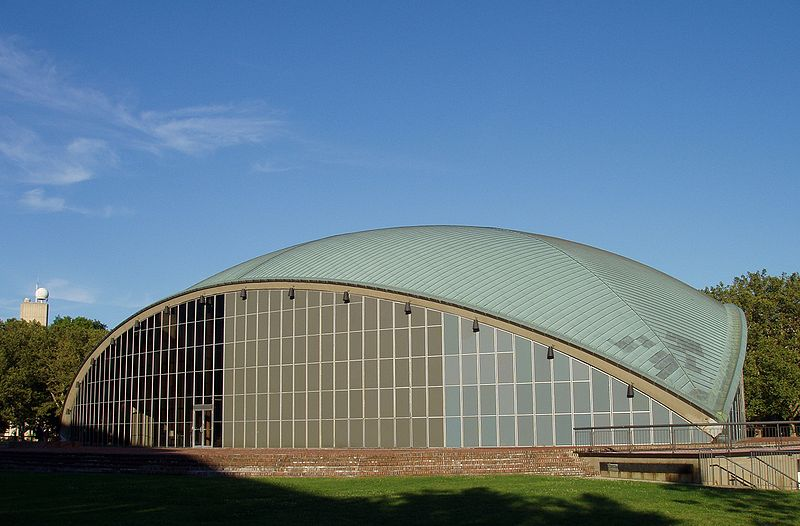
\includegraphics[width=4in]{images/kresge_auditorium.jpg}
\caption[The Kresge Auditorium]{The Kresge Auditorium on the MIT campus in Cambridge, Massachusetts is an example of the problem thin-shell
structures can cause when not designed properly.  Since the roof is octanispeherical rather than catenarian, the forces do not travel as
intended and the building has been plagued with structural problems since its construction.  ``Kresge Autidorium", Eero Saarinen, photo
taken by Ibn Battuta \url+http://en.wikipedia.org/wiki/File:Kresge_Auditorium,_MIT_(view_with_Green_Building).JPG+}
\label{fig:kresge_aud}
\end{figure}

\begin{figure}
\centering
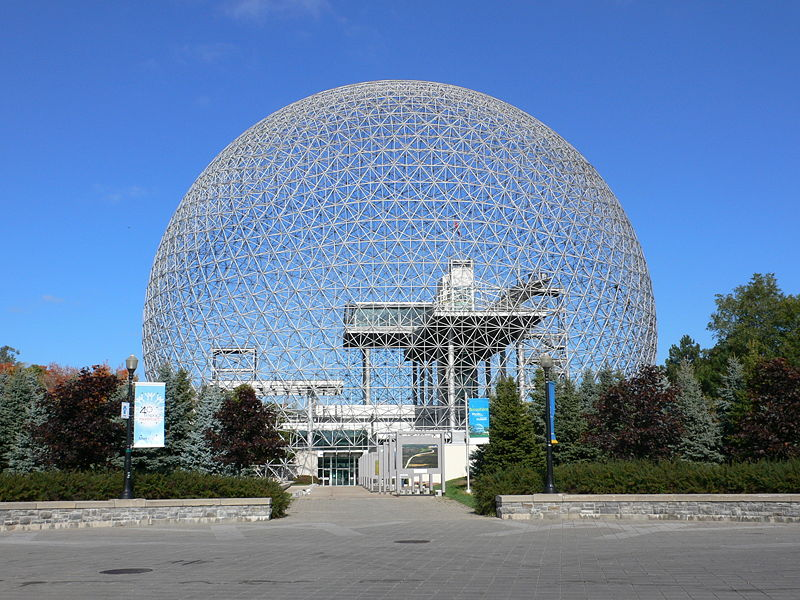
\includegraphics[width=4in]{images/montreal_biosphere.jpg}
\caption[The Montreal Biosphere]{The Montreal Biosphere is an example of a lattice-based thin-shell structure, which relies on a lattice of
struts to support the huge expanse of the dome.  ``Montreal Biosphere", Richard Buckminster Fuller, photo taken by Philipp Hienstorfer
\url+http://en.wikipedia.org/wiki/File:Biosphere_montreal.JPG+}
\label{fig:montreal_bio}
\end{figure}


\subsection{Structural Stability} \label{sec:stability}
The core concept for structural stability for masonry buildings is the concept of lines of thrust.  Lines of thrust are lines that can be drawn
in the direction of the forces neighboring elements of the structure impart on one another.  If all the discrete forces are connected together
into a generalized curve, the traditional lines of thrust are obtained.
In order for a building to stand up, these lines of thrust must pass through structural elements.  As can be seen in Figure \ref{fig:arch_lines},
traditional arches must be rather thick to contain the lines of thrust produced by their weight.  However, a catenary arch can be built
much thinner for the same stability, as it contains the line of thrust exactly.  For example, the Gateway Arch in St. Louis, Missouri (Figure
\ref{fig:gateway_arch} is constructed in the shape of a catenary arch.  This allows it to be thin and elegant while remaining very stable.
To extrapolate the concept of lines of thrust to entire buildings, traditional construction methods require very thick elements such as walls
and columns to be used in order to keep the lines of thrust within a building's structural elements.  This is especially true of large masonry
structures such as cathedrals.  However, if the shape of the building is instead matched to
the shape of the lines of thrust, the structural elements can be much thinner, since they only need to support the direct compressive force.
\begin{figure}
\centering
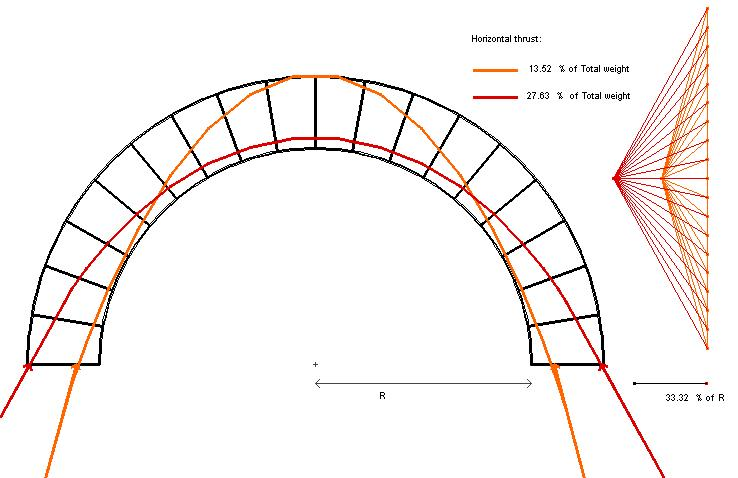
\includegraphics[width=4in]{images/arch.png}
\caption[Lines of thrust]{This figure shows the lines of thrust within a standard masonry arch.  As can be seen from the minimum and maximum
lines, the arch must be rather thick in order to contain the lines of thrust, thereby wasting material.  This image is a screenshot of the
"Interactive Thrust" tool created by John Ochsendorf.  It can be found at \url+http://web.mit.edu/masonry/interactiveThrust/applets/applet01.html+}
\label{fig:arch_lines}
\end{figure}

\begin{figure}
\centering
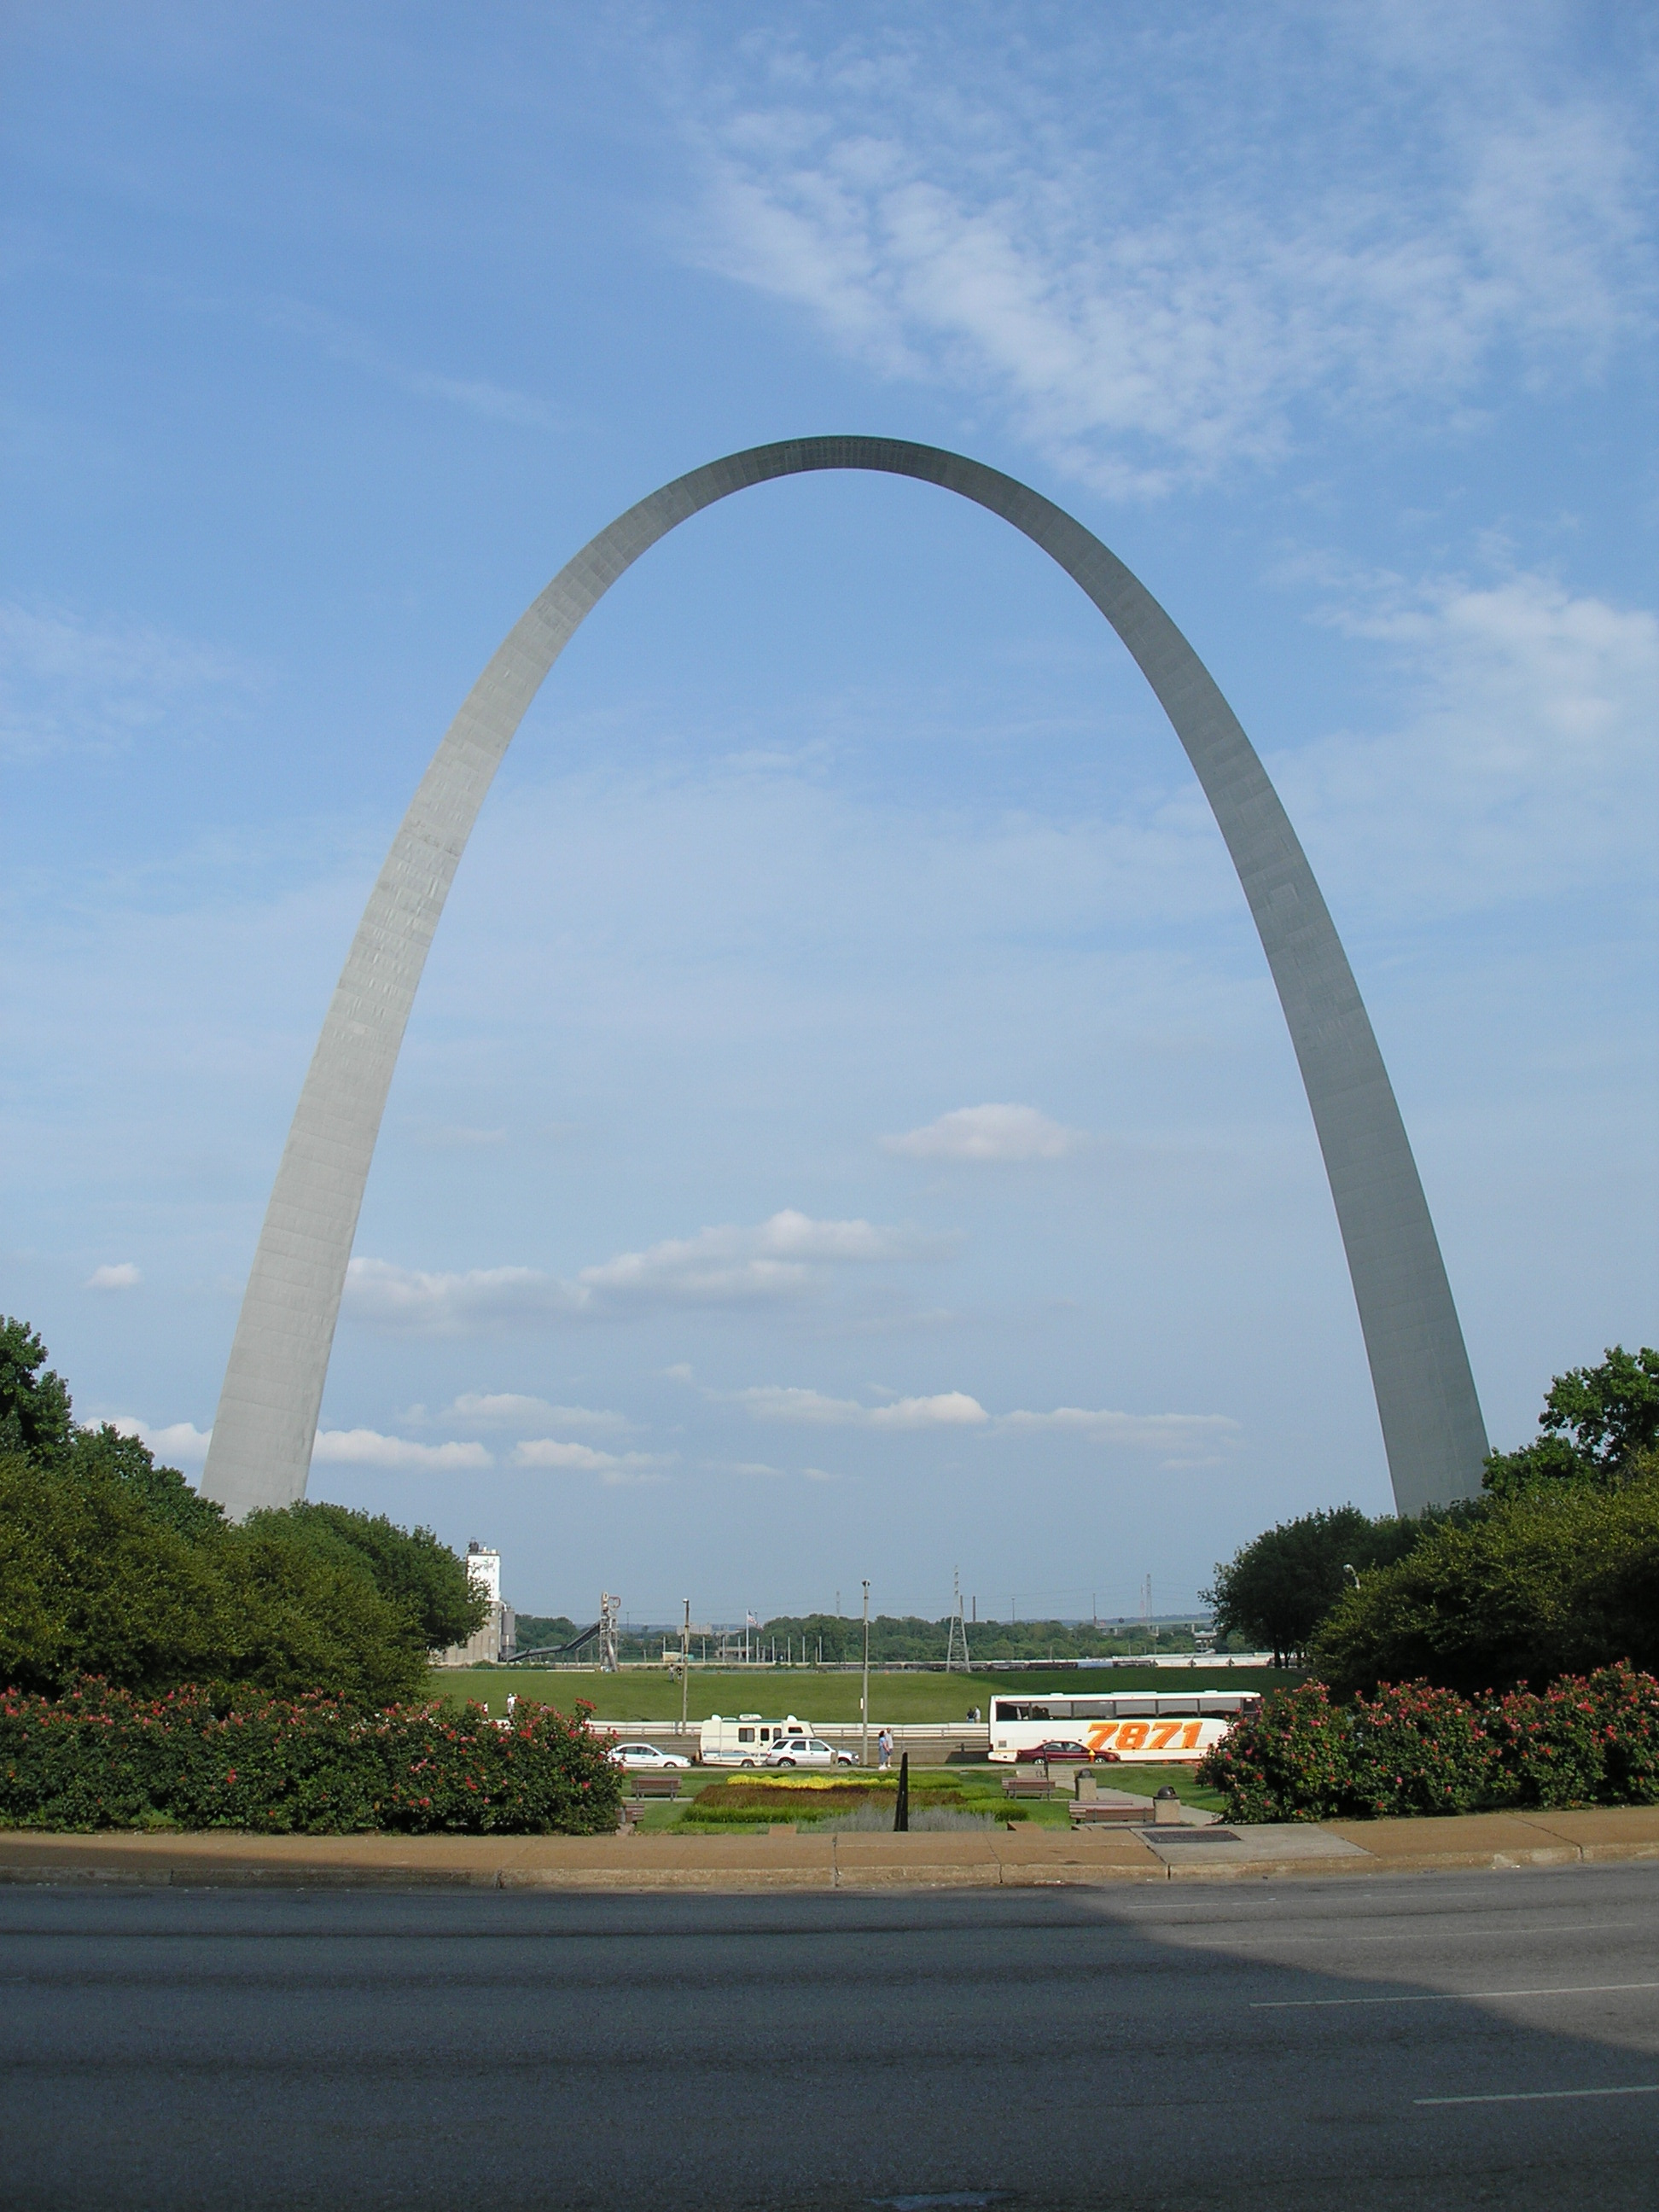
\includegraphics[height=3.5in]{images/gateway_arch.jpg}
\caption[The Gateway Arch]{The Gateway Arch in St. Louis, Missouri is an example of a catenary arch.  Since the lines of thrust travel directly
through the structure of the arch, it can be built very thin.  ``Gateway Arch", Eero Saarinen, photo taken by David K. Staub
\url+http://en.wikipedia.org/wiki/File:Gateway_Arch.jpg+}
\label{fig:gateway_arch}
\end{figure}

\subsection{Catenary} \label{sec:catenary}
The term for the shape that lines of thrust tend to take is called a catenary.  A catenary is a curve described by the function
\[y=a cosh(\frac{x}{a})\]
where cosh is the hyperbolic cosine function.  Several examples of catenaries can be seen in Figure \ref{fig:catenary}.  In addition to being
an interesting mathematical figure, the catenary is the shape taken by a cable, rope, or chain suspended at both ends, as seen in Figure
\ref{fig:hanging_chain}.  Since this is the shape formed by a freely hanging object under pure tension, it is not surprising that if inverted,
it is similarly stable under pure compression.  For this reason, catenary arches and catenary shells are the primary building blocks of
thin-shell structures.  One very important thing to note is that a catenary is only the optimal shape when the chain or arch is evenly loaded.
If there is an uneven load, for example if the arch has a decorative mass at some point or if a secondary arch rests on another arch, the
catenary is not the optimal shape, as seen in Figure \ref{fig:compound_catenary}.

\begin{figure}
\centering
\subfloat[]{
  \label{fig:catenary}
  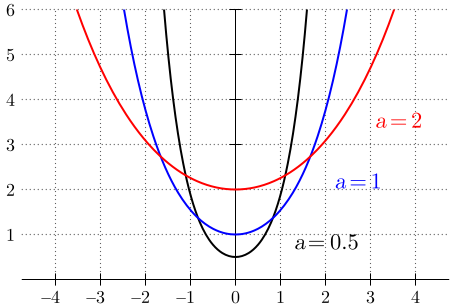
\includegraphics[height=1.7in]{images/catenary.png}
}
\subfloat[]{
  \label{fig:hanging_chain}
  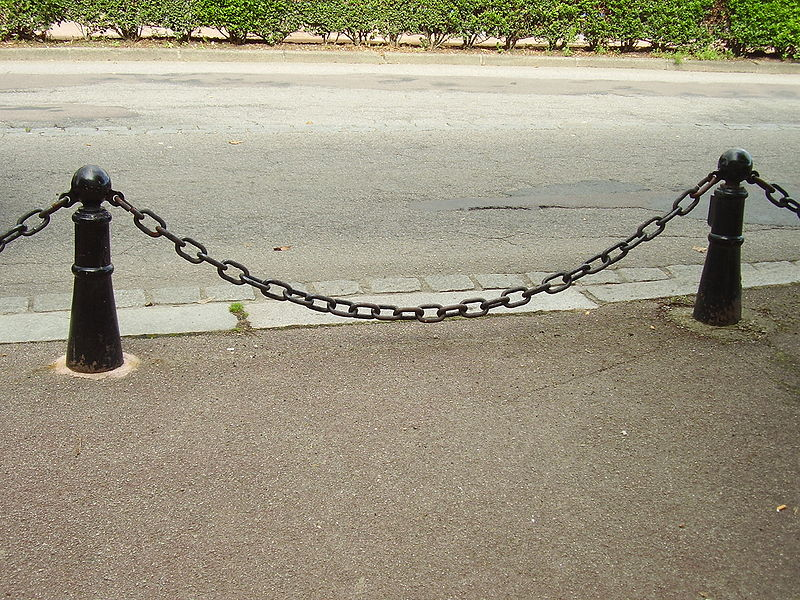
\includegraphics[height=1.7in]{images/hanging_chain.jpg}
}
\caption[Example catenary curves]{Image (a) shows a few catenary curves for various values of a.  ``Catenary Curves", image created
by Geek3, \url+http://en.wikipedia.org/wiki/File:Catenary-pm.svg+  Image (b) shows a natural catenary formed by a freely hanging chain.
"Hanging Chain", photo taken by Kamel15, \url+http://en.wikipedia.org/wiki/File:Kette_Kettenkurve_Catenary_2008_PD.JPG+}
\end{figure}

\begin{figure}
\centering
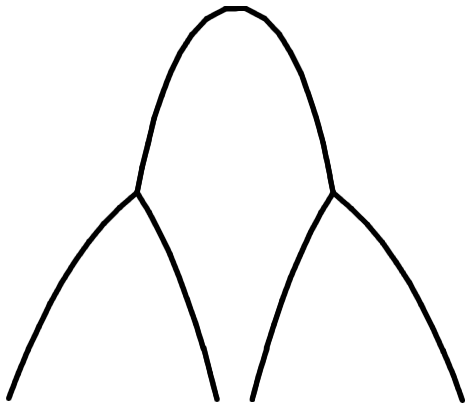
\includegraphics[width=2.25in]{images/compound_catenary.png}
\caption[A composite catenary structure]{This image shows the necessary deformation of supporting catenary arches when a third arch is placed
on top of them.}
\label{fig:compound_catenary}
\end{figure}

The shape of the catenary has been used by many architects.  One example mentioned earlier is the Gateway Arch in St. Louis, Missouri, designed by
the Finnish-American architect Eero Saarinen, seen in Figure \ref{fig:gateway_arch}.  However, the shape has also been used as an integral design
principle for much larger and more complex structures.  Hanging chains have been used by a number of architects to design structures for stability and
aesthetics.  One famous user of hanging chains is Antoni Gaud\'{i}, whose catenary-rich projects include such Barcelona landmarks as the Casa Mil\`{a}
(Figure \ref{fig:casa_mila}), Park Guell (Figure \ref{fig:parc_guell}), and Sagrada Familia (Figure \ref{fig:sagrada_familia}).  The works of Antoni
Gaud\'{i}, his design methods, and his aesthetic style are beautifully photographed, discussed, and analyzed in Rainer Zerbst's
\underline{Antoni Gaud\'{i} The Complete Buildings}\cite{zerbst85gaudi}.  Figure \ref{fig:gaudi_model} shows one of the models Gaud\'{i} used in
creating these graceful structures.

\begin{figure}
\centering
\subfloat[]{
	\label{fig:casa_mila_ext}
	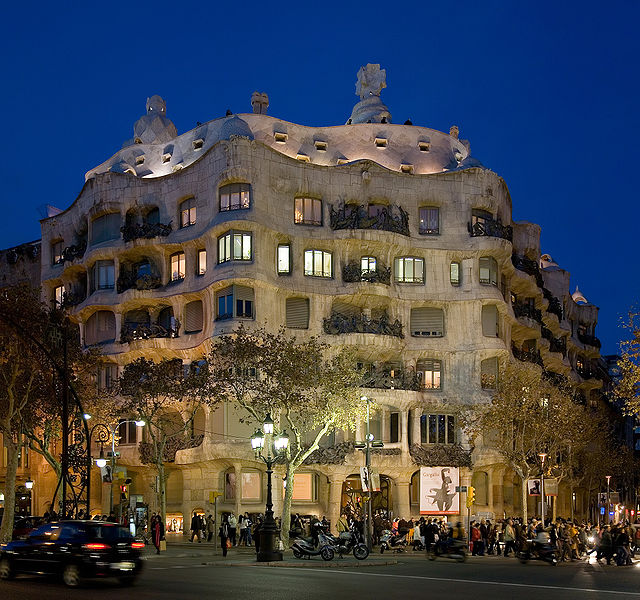
\includegraphics[height=3in]{images/casa_mila_ext.jpg}
}
\subfloat[]{
	\label{fig:casa_mila_arch}
	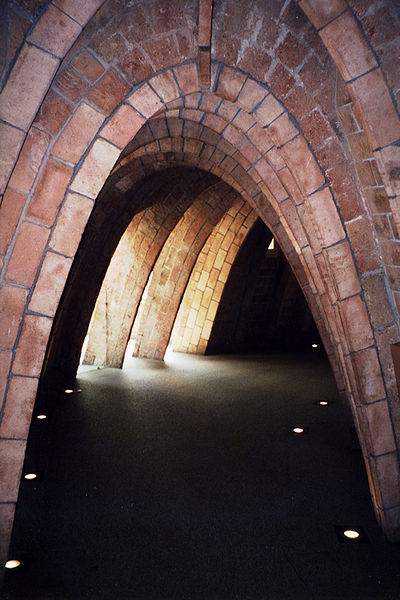
\includegraphics[height=3in]{images/casa_mila_arch.jpg}
}
\caption[Casa Mil\`{a}, Barcelona, Spain]{Image (a) shows an exterior view of Casa Mil\`{a}, one of Antoni Gaud\'{i}'s stunning buildings in
Barcelona, Spain. ``Casa Mil\`{a}", Antoni Gaud\'{i}, photo taken by David Iliff
\url+http://en.wikipedia.org/wiki/File:Casa_Mil\`{a}_-_Barcelona,_Spain_-_Jan_2007.jpg+ Image (b) is of the catenary arches under the terrace
of Casa Mil\`{a}. ``Casa Mil\`{a}", Antoni Gaud\'{i}, photo taken by Error, \url+http://en.wikipedia.org/wiki/File:LaPedreraParabola.jpg+}
\label{fig:casa_mila}
\end{figure}

\begin{figure}
\centering
\subfloat[]{
	\label{fig:parc_guell_ent}
	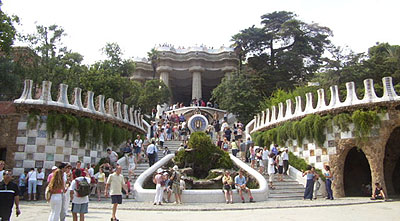
\includegraphics[height=2in]{images/parc_guell.jpg}
}
\subfloat[]{
	\label{fig:parc_guell_arch}
	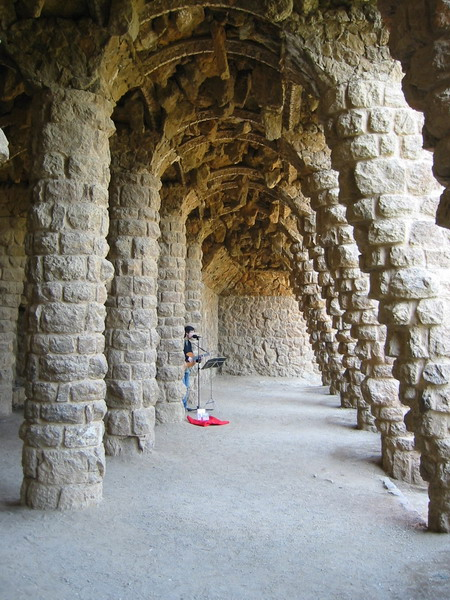
\includegraphics[height=2in]{images/parc_guell_arch.jpg}
}
\caption[Parc Guell, Barcelona, Spain]{Image (a) shows the entrance to Parc Guell in Barcelona.  ``Parc Guell Entrance", Antoni Gaud\'{i}, photo
taken by Montrealais \url+http://en.wikipedia.org/wiki/File:Parcguell.jpg+  Image (b) shows the columns supporting the roadway that runs past the
park.  These columns form an offset catenary, which is asymmetric because the loading of the arch is asymmetric. ``Parc Guell", Antoni Gaud\'{i},
photo taken by Rapomon, \url+http://en.wikipedia.org/wiki/File:Parc_Guell_10.jpg+}
\label{fig:parc_guell}
\end{figure}

\begin{figure}
\centering
\subfloat[]{
	\label{fig:sagrada_familia_nativity}
	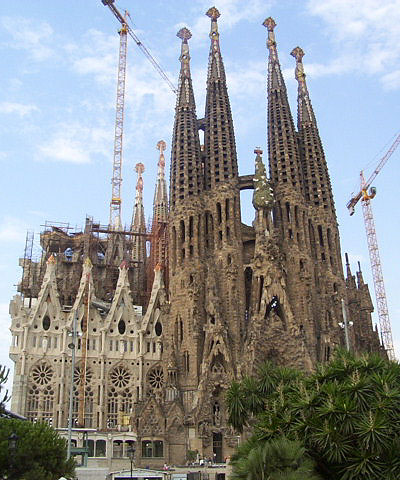
\includegraphics[width=2.5in]{images/sagrada_familia_nativity.jpg}
}
\subfloat[]{
	\label{fig:sagrada_familia_columns}
	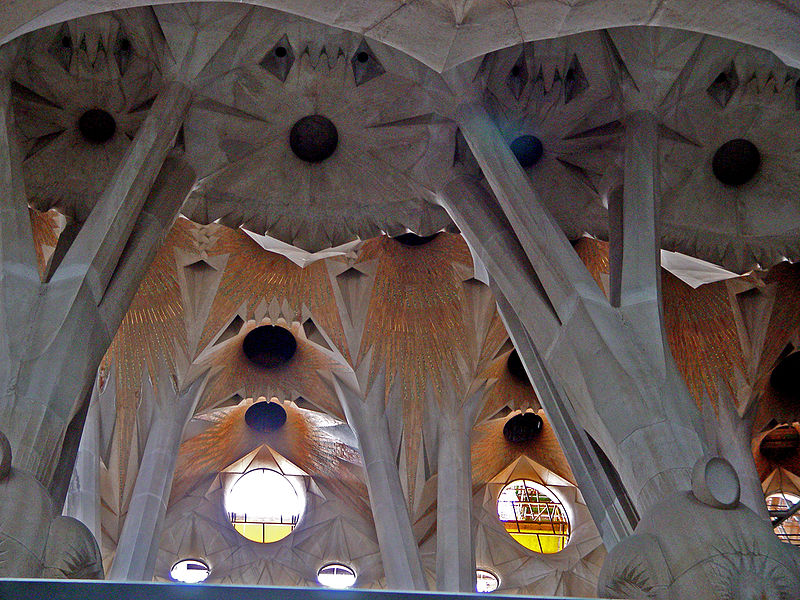
\includegraphics[width=3in]{images/sagrada_familia_columns.jpg}
}
\caption[Sagrada Fam\'{i}lia, Barcelona, Spain]{Image (a) shows the nativity fa\c{c}ade of Antoni Gad\'{i}'s masterpiece, Sagrada Fam\'{i}lia,
slated to be completed some time after 2026.  ``Sagrada Fam\'{i}lia", Antoni Gaud\'{i}, photo taken by Montrealais,
\url+http://en.wikipedia.org/wiki/File:Sagradafamilia-overview.jpg+  Image (b) shows the strucutral columns that are possible when
designing with catenaries in mind.  Rather than the monolithic columns found in most gothic cathedrals, Gaud\'{i} has whittled away the nonessential
stone to reveal the core load-bearing elements.  This results in a gracefully arcing column that supports the huge structure as well as a monolithic
column would have.  ``Sagrada Fami\'{i}lia", Antoni Gaud\'{i}, photo taken by Etan J. Tal,
\url+http://en.wikipedia.org/wiki/File:SagradaFamiliaRoof.jpg+}
\label{fig:sagrada_familia}
\end{figure}

\begin{figure}
\centering
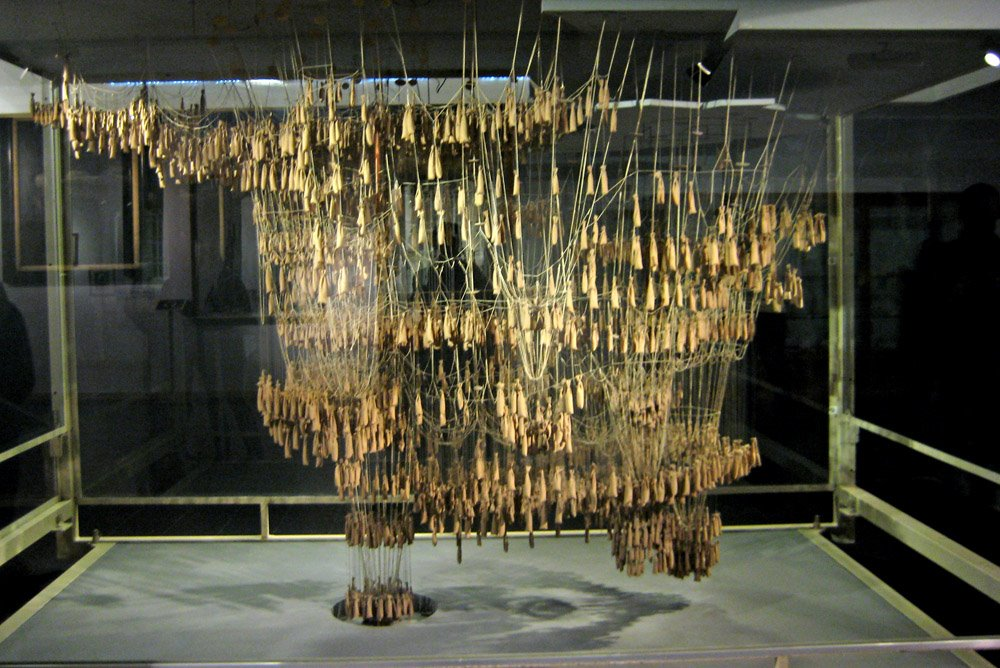
\includegraphics[width=4in]{images/gaudi_model.jpg}
\caption[A hanging model used by Gaud\'{i}]{This is a photo of one of the hanging models used by Antoni Gaud\'{i} to understand the forces in
the buildings he constructed.  The bags are full of small lead weights which are proportonal to various structural elements and ornaments in
the planned building.  The strings holding them together are the necessary columns, arches, and other core structural elements that will make
up the building.  ``Hanging model", Antoni Gaud\'{i}, photo taken by Pamela Angus, 
\url+http://2.bp.blogspot.com/_PZOVPTsrTJ0/SR7z2F_h93I/AAAAAAAAAls/hAv1--bslzQ/s1600-h/Gaudi+model.jpg+}
\label{fig:gaudi_model}
\end{figure}

Another architect who is famous for his use of catenary shells in his thin-shell structures is Heinz Isler.  A civil engineer from Switzerland,
Isler designed some very beautiful and elegant structures using the simple tools of cloth and water.  Since a sheet of cloth will behave as an
interconnected set of hanging strings, it can be used to create catenary shell structures.  What Isler did was to take the shape a sheet of cloth
formed when suspended and freeze it by soaking the cloth evenly with water.  The resulting frozen structure was then inverted and measured very
accurately with a device he created.  Once these measurements had been taken, he built forms and poured the shell using standard concrete
construction techniques.  The resulting buildings, such as those in Figure \ref{fig:isler_service}, are elegant, graceful structures with an
exquisite simplicity of form and conservation of material.

One drawback to the thin-shell structure work done by Gaud\'{i} and Isler is that the design process is very time-consuming.  The amount of time
it takes to create a hanging model from strings and lead shot or freeze a cloth shell is prohibitive to the fast-paced, quick turnaround time of
the modern architecture world.  Fortunately, both hanging chains and cloth are rather easy to simulate, and therefore software can be created to
allow these designs to be rapidly prototyped, tweaked, and refined on the computer.

\clearpage
\chapter{RELATED WORKS}
\section{Procedural Modeling}
In ``Procedural Modeling of Strucutrally-Sound Masonry Buildings"\cite{whiting:2009}, Whiting, Ochsendorf, and Durand explore
the possibilities of creating existing or novel structures procedurally.  They began by creating a grammar
which can be used to construct masonry buildings.  Arches, buttresses, domes, and vaults are some of the
structural elements which are then combined in their software.  These grammar elements are assembled into
a structure through a procedural algorithm which cuts windows in walls and assembles
all the various masonry elements of the building.  Once the initial configuration is
generated, the software runs static analysis on the building.  If it is feasibly stable, the program is
done.  If not, the program determines a measure of infeasibility, which is a measure of how far away from
stable a structure is.  The static analysis only allows for compressive forces, as the tensile strength of
masonry elements is close to zero.  Friction is also modeled, allowing for some shear.  Once the measure
of infeasibility is calculated, a parameter search is conducted iteratively, searching the parameter space
for a stable configuration.  Depending on the application, this stable configuration will take into account
a factor of safety.  The more likely a structure is to have changing loads, the higher a factor of
safety is needed.  For example, a bridge needs a higher factor of safety than a cathedral.  In the event
that there is no feasible configuration for a structure, the least infeasible structure is returned and the
user is required to add new structural elements.

In ``Creating Models of Truss Structures with Optimization"\cite{Carnegie02creatingmodels}, Smith, Hodgins, Oppenheim, and Witkin propose
a method of creating trusses procedurally.  This work allows the user to define several anchor points
and loads for a truss, then have the software automatically generate a truss.  In this work, the risk
of pieces falling apart is not an issue as it was in the previous paper.  The primary failure method
in this case is buckling, since all forces are axial.  Therefore, the core of the algorithm is a
multivariable optimization with constraints.  The algorithm attempts iteratively to minimize weight
while ensuring that none of the members will fail, either in tension or compression.

My work had initially intended to go in this direction, using static analysis of structures within
Google Sketchup.  However, Sketchup proved to be a poor environment for the program I wanted to write, so
the project was moved to a standalone application and the focus shifted to thin-shell structures.  With this
shift in focus, the simulation method shifted from static analysis of structures to dynamic simulation of
structure using techniques from cloth simulation.  This simulation was designed to imitate the behavior of
hanging chains or cloth.

Hanging chains and cloth have been used by a number of architects in the design of structures.  In
\underline{Finding Form}\cite{otto95findingform}, Otto and Rasch discuss a number of natural inspirations of form, among which
is hanging chains.  They show that a naturally hanging square-mesh chain net will form the shape of
traditional Asian roofs, while inverting chain nets suspended differently will yield the ideal structure
for arches, domes, and vaults.  While this has been known for some time, it is comforting to see
well-documented, carefully constructed pictures of these structures.  As was discussed in\ref{sec:catenary},
Antoni Gaud\'{i} and Heinz Isler used thin-shell structures and hanging chains similar to those described in
\underline{Finding Form} constantly as an integral part of their design processes.

\section{Cloth Simulation}
Much work has been done in the field of cloth simulation.  In ``The Synthesis of Cloth
Objects"\cite{weil86synthcloth}, Jerry Weil lays the groundwork for much of the future of cloth simulation.
Weil describes a method of surface generation that draws catenaries between points in order to approximate
the surface of a hanging cloth, then iteratively relaxes the surface to more accurately represent a
naturally draping piece of cloth.

Further work on the simulation of elastic bodies was done by Terzopoulos, Platt, Barr, and Fleischer in
"Elastically Deformable Models"\cite{terzopoulos87elastic}.  This paper yields results that are applicable
much more generally than simply cloth simulation.  The elastic model that is created can be used for cloth,
solids, and other elastic manifolds.  By summing the internal strain energies and energies applied by
external forces such as gravity or wind then integrating the resulting equations numerically, an animation
of these deformable models can be created.

These early examples of cloth simulation are expanded upon by Volino, Courchesne, and Thalmann in ``Versatile
and efficient techniques for simulating cloth and other deformable objects"\cite{volino95cloth}.  In this
paper, the internal shear and bending strain energies and external forces are augmented by further collision
energies, such as self-collision.  This algorithm is robust enough to simulate such complex situations as
cloth tumbling in a dryer and a dress draping around a walking human.

In ``Deformation constraints in a mass-spring model to describe rigid cloth behavior"\cite{provot95deformationconstraints},
Xavier Provot describes a method for cloth simulation on which the simulation used in this thesis is based.
A cloth consisting of a mesh of masses and springs is subjected to external forces such as gravity.  These
external forces are combined with internal spring forces to obtain the total force on each point.  However,
this simulation method results in overstretching, the cloth behaving more like putty than cloth.  Therefore,
Provot implements a correction step, wherein the points are brought closer together if they have stretched
farther than some allowed amount.  This correction prevents the cloth from stretching farther than reality
would allow.

Far more advanced cloth simulation methods have been developed more recently which are not implemented in
this project but which are planned for future work.  In ``Large Steps in Cloth Simulation"\cite{baraff98largesteps},
Baraff and Witkin propose an implicit simulation method which is the basis for most modern cloth simulation.
The same shear and bending forces used in the earlier methods, as well as gravity and other external forces
are applied to the cloth, but instead of being explicitly integrated, an implicit integration method employing
sparse matrices is employed.  The sparse matrix of equations resulting from the internal and external forces
is solved using a modified Conjugate Gradients method that can operate on asymmetric systems.

\section{Other Software}
There is a large variety of software available for structural analysis, architectural modeling, and even
catenary design.

Foremost in the field of finite element analysis is NASTRAN\cite{NASTRAN}.  Originally developed for NASA in
the 1960s, NASTRAN is one of the most advanced finite element analysis packages on the market.  Able to
analyze both static and dynamic systems in a wide variety of failure modes, NASTRAN is the software
of choice for analysis of parts and systems for any mechanical application.  While NASTRAN is very good
at what it does, it gives information on a lower level than is relevant for most architectural applications.
Furthermore, it is not a real-time application.

Another piece of software that is relevant in architectural design is Dr. Frame 3D\cite{drframe}.  This
software is more useful in architectural design, as there is an interface for building frames and structures.
Once constructed, the user can apply loads and see the resulting deformations, moments, and other relevant
visualizations.  However, as with standard architectural CAD packages such as Rhino\cite{rhino} and
AutoCAD Architecture\cite{autocad}, it is tedious to construct an accurate catenary, as there are no
tools for easily creating an arbitrary stable shell.

One tool that is useful in creating arbitrary shell structures is CADenary\cite{cadenary}.  With this tool,
users can attach endpoints of strings and sheets to points on a grid or points on existing strings and sheets.
Interesting shells can be made, but once points are placed they are fixed, which is disadvantageous for
iterative design.  In his paper ``Linking Hanging Chain Models to Fabrication"\cite{kilian05cadenary}, Axel Kilian
discusses his tool in finer detail, detailing its features and the design process behind it.

(Any other software I'm forgetting?)


\chapter{BACKEND / SIMULATION ALGORITHM (BETTER TITLE GOES HERE)}
\section{Data Structure}
The primary data structure is the cloth object.  This object contains an array of points which are connected to each other through springs.
Each point has a list of structural and shear springs that are connected to it.  These springs know what their resting length is and have
a pointer to the point at the other end.  These springs exert forces on the points to which they are connected based on stiffness constants
which are determined when the cloth is loaded.  The other attribute that points can have is the ``fixed" attribute.  Fixed points are
attached to the ground and can be moved only by the user manipulating the points in the floorplan pane.

This data structure taken as a whole represents a discrete mesh, upon which a simulation can be run.  Figure \ref{fig:wireframe} shows
the wireframe view of a model within the simulator.  The lines in the image are the springs connecting points, and each place where
the points meet is a discrete mass.  Each point has both structural and shear springs coming from it, and the forces applied by these
springs together with the force of gravity give the shell its stable shape.  In Figure \ref{fig:wireframe_detail}, the forces acting on
a point are annotated.  The green arrow represents gravity, the red arrows mark the structural springs, and the blue arrows mark the
shear springs.  It may seem curious that gravity is applying a force up, but the reason for this is to make the structure easier to
comprehend.  While the simulator is constructing a hanging chain model, the architect is interested in the final shell, which is
the hanging chain model inverted.  Therefore, since this is a simulator, gravity can easily be inverted within the simulation to
obtain accurate results in an easily visualized form.  The structural forces are the hanging chains in the simulation, while the
shear forces are the forces that would be present in an actual structure keeping the structure from collapsing due to a lack of
constraints.

\begin{figure}
\centering
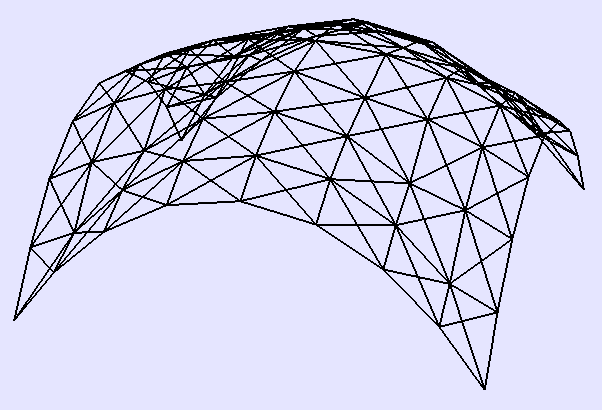
\includegraphics[width=3in]{images/wireframe.png}
\caption[A wireframe of a simulated model]{This image shows a wireframe in the simulator.  The lines represent springs, while the points
where they meet are the discrete points of mass.}
\label{fig:wireframe}
\end{figure}

\begin{figure}
\centering
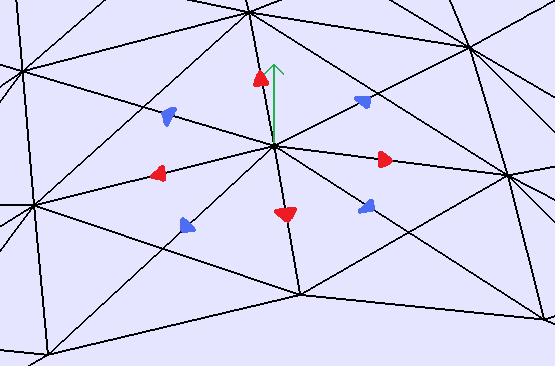
\includegraphics[width=3in]{images/wireframe_detail.png}
\caption[Detail of a wireframe of a simulated model]{This image shows annotations on a portion of a wireframe.  In this image, green is
gravity, red is structural forces, and blue are shear forces.}
\label{fig:wireframe_detail}
\end{figure}

\section{Algorithm}
In the interest of having short timesteps and thus a higher framerate and better interactivity, a second order explicit Euler integration
method was implemented for the simulation.  Explicit Euler integration finds the tangent line of the function at the current point, then
moves in that direction for a timestep and repeats.  
At each step of the simulation, the system iterates over all the vertices in the shell, and for each vertex calculates the forces acting
upon it.  As shown above, the forces acting upon any given point are gravity and the spring force exerted by all connected points.  Once
the forces have been calculated, the algorithm divides the forces by the masses of the points, yielding an acceleration.  The acceleration
can by multiplied by the time step to obtain a velocity, which is again multiplied by the time step to get the new position of the point.
However, this single-step explicit integration is very imprecise.  If the timestep or forces involved are very large, the result will
have a large amount of error, which can cause instability, inaccuracy, or oscillations.  To combat this problem, a further calculation
is performed which calculates the midpoint of the original step and takes an additional half-step from that point.  This second-order
integration method is much more stable, so much larger timesteps can be taken, as shown in Figure \ref{fig:euler_integration}.  A
fourth-order system was created, but despite its stability, each step took too long for it to be useful in an interactive simulation.

\begin{figure}
\centering
\subfloat[]{
	\label{fig:euler1}
	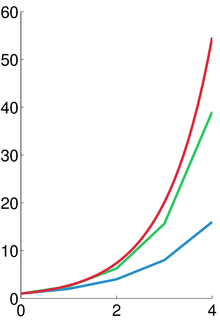
\includegraphics[width=2in]{images/euler1.png}
}
\subfloat[]{
	\label{fig:euler.25}
	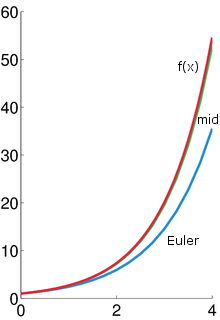
\includegraphics[width=2in]{images/euler25.png}
}
\caption[Euler integration]{These images show the error that is present in explicit Euler integration.  The red line is the target,
the blue line is first order Euler integration, and the green line is the midpoint method.  Image (a) has a timestep of 1,
while image (b) has a timestep of 0.25.  As can be seen, the smaller timestep results in lower error, but error is still present.}
\label{fig:euler_integration}
\end{figure}

After the Euler integration is performed, overstretched springs are shortened in two ways.  First, the saved original length of the
spring is shortened so that the force pulling it back towards the original shape will be higher.  This correction will reverse and
increase the original length if the overstretched spring becomes overcontracted.  Secondly, the points will be adjusted such that
a hard cap is enforced on the lengths of the springs in order to prevent the deformation from becoming too severe, as detailed
in\cite{provot95deformationconstraints}.  While a higher spring constant would also cause the springs to stay shorter in general,
if the constant becomes too large, the forces operating within the cloth will become very large and the simulation will become
unstable.  The only way to combat an unstable simulation using the explicit Euler method is by shrinking the timestep, which
will slow down the simulation.  In order for the simulation to be interactive, a large enough timestep must be used that a stiff
cloth is not feasible, thus requiring the use of these correction techniques.

This simulation finds equilibrium when the forces exerted by the springs balance the force of gravity and the velocities of the particles
are all zero.  Depending on the number of points in the shell and the changes made to the shape since it was last in equilibrium, the
simulation could take anywhere from a few seconds to a few minutes to reach this resting state.  Figure \ref{fig:wireframe_sim} shows
the motion of a shell as it progresses from an initial mesh to a stable thin-shell configuration.

\begin{figure}
\centering
\subfloat[]{
	\label{fig:wireframe_sim1}
	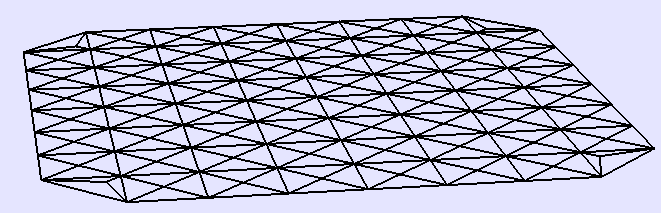
\includegraphics[width=3in]{images/simframe1.png}
}
\subfloat[]{
	\label{fig:wireframe_sim2}
	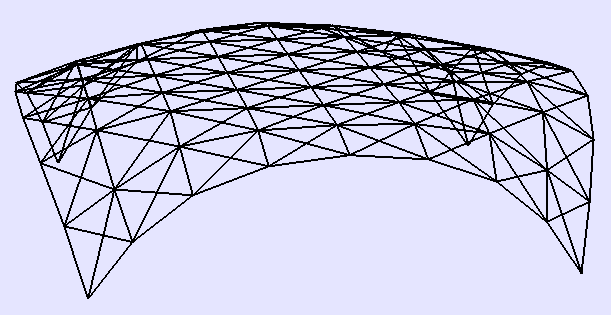
\includegraphics[width=3in]{images/simframe2.png}
}\\
\subfloat[]{
	\label{fig:wireframe_sim3}
	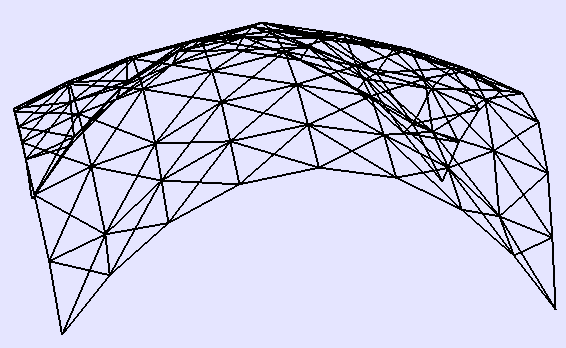
\includegraphics[width=3in]{images/simframe3.png}
}
\subfloat[]{
	\label{fig:wireframe_sim4}
	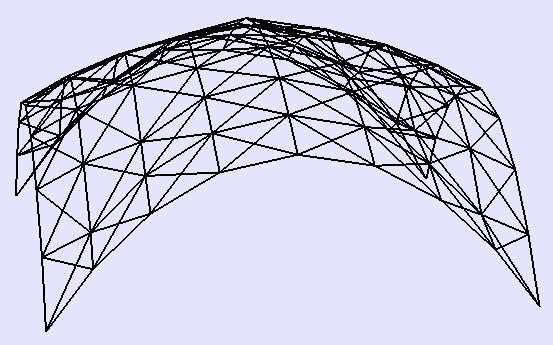
\includegraphics[width=3in]{images/simframe4.png}
}
\caption[Simulation frames]{These images show the motion of a shell as it is subjected to the simulation.  (a) is the starting position,
(b) shows the shell as the points begin to ``fall", (c) shows the shell as the points stop their free-fall, and (d) shows the equilibium
position.}
\label{fig:wireframe_sim}
\end{figure}

(Insert table/graph of performance for different numbers of points here)

\section{Advantages}
There are numerous advantages to using an explicit midpoint integration method over other methods.  Midpoint has a considerable stability
advantage over a first-order explicit integration, and is faster per frame than a fourth order Runge-Kutta integration or implicit
integration.  The stability increase over a first-order integration has the obvious benefit of being able to take considerably larger
time steps.  A fourth order Runge-Kutta solver was implemented, but the advantage of increased stability and associated larger timestep
was offset by the long computation time per frame.  When implemented, the 4th-order solver took much too long per frame to be practical
for an interactive simulation on reasonably large meshes.

The spring correction allows for the imitation of very stiff springs without requiring very small timesteps.  For a relatively small
execution time, the structure can be corrected in such a way that it remains structurally correct and avoids overstretching.

\section{Disadvantages}
The primary disadvantage to an explicit solver rather than an implicit solver is that the timestep is limited.  However, while an
implicit solver can theoretically operate with arbitrarily large timesteps, the computation tradeoff is not favorable.  Furthermore,
the timestep used in the current simulation is large enough that the user does not grow impatient waiting for the structure to reach
equilibrium, nor is it short enough that the user cannot react to the motion of the shell.  An ancillary disadvantage to the
explicit solver is the necessity of correction methods to prevent overstretching.  However, this disadvantage is again offset by the
fact that even with the correction methods, the explicit solver is faster than an implicit solver.



\chapter{USER INTERFACE}

\section{Layout}
As can be seen in figure \ref{FIGURE_screenshot}, there are 3 main panels in the design tool.  On the left is the viewing panel, where the structure
is shown in 3D.  This view can be rotated, zoomed, and panned to give the architect the view they need.  There is no actual interaction with the
structure in this panel; all of the interaction is done via the two right-hand panels.  The top-right panel is the floorplan panel.  This panel
contains a point for each point of the structure that is in contact with the ground.  These points can be moved around in order to modify the shape
of the structure to fit the architect's vision.  The bottom-right panel is the grid panel.  This panel shows all the vertexes of the structure in 2D.
This panel can be used to disable points, creating voids in the structure.  It can also be used to associate different points in the shell with certain
points in the floor plan.  This is most useful when adding new points to the floor plan, allowing the architect to define a new point of support on the
fly.  Together, these windows allow the architect broad control over the design of their structure, while the tool works in the background to keep the
shape of the structure optimal.
\begin{figure}
\resizebox{5in}{!}{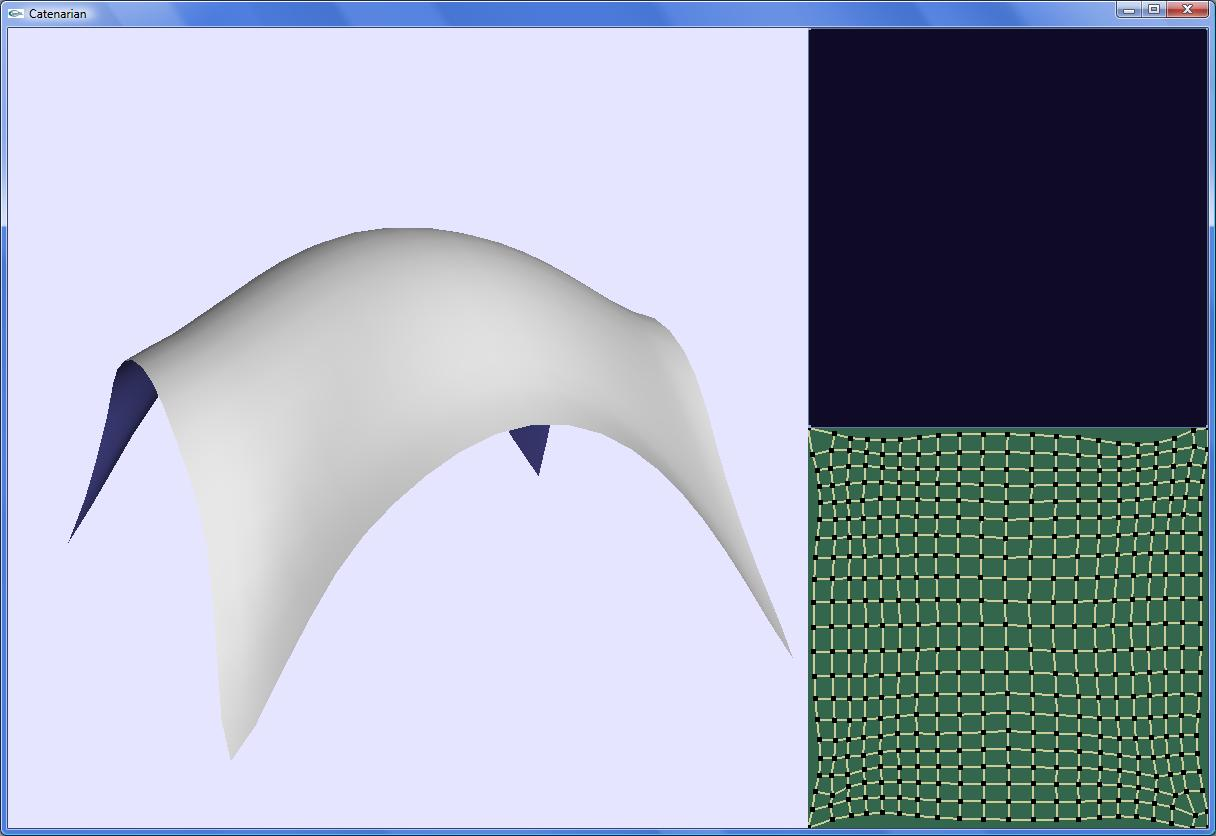
\includegraphics{images/screenshot.png}}
\caption{A screenshot of the tool}
\label{fig:screenshot}
\end{figure}


\chapter{USER STUDY}
\section{Design of the Study}
When designing the user study for this tool, the first consideration was what I wanted to get out of the study.  Being that this is
a design tool and not a scientific tool, the results of a user study were liable to be rather subjective rather than provide any hard
data.  Fortunately, subjective is exactly what I wanted from this study.  My goal is to provide a useful tool that conforms to users'
expectations and provides the functionality that they expect from it.

\section{Observations}
The first user I had in to use the software was an architecture student who was very excited about the software.
The first thing I noticed when he started using the software was that he tried to zoom with the mouse wheel.  That's a feature that
should be added.  Mouse wheel scrolling is a common functionality that shouldn't be too hard to implement.

As he continued to use the software and get more comfortable with it, he noted that having left-click have an immediate action was not
what he was used to. Most architectural software allows the user to select points with the left mouse button, then right-click to
bring up the interaction menu.  A standardization would be a good idea.  This is especially true in the floorplan window, where
left-clicking places a new point, which is not what the user wants when they miss selecting a point by a few pixels.  On a related
note, an undo feature would be very welcome.  While it would be less of an issue if accidental left-clicks did not create points,
an undo feature would still help the user to revert changes, whether this reversion stems from error or indecision.

Something that became very clear to me as the user continued to use the software is that the current implementation of the grid
interface is a bit clunky.  Firstly, new points should automatically associate with the closest point in the grid.  That's almost
always what the user does next, and it saves them from having to guess which point is the closest, which is especially useful in a
high-density grid.  However, the real problem with grid association is the snapping.  Since the floorplan point does not move when
it is associated with a new grid point, the mesh is forced to warp, sometimes drastically, to acquiesce to the user's request.
I am not sure what the best approach to this would be.  Moving the floorplan point to match the grid does not make much sense,
since that's not usually what the user is trying to do.  Moving them both to the average also does not make a lot of sense.
I suspect, however, that the main problem with the snapping is less that it snaps and more that it surprises the user when it
happens.  I think having a less immediate interface would help with this.  For example, if rather than left-click associating the
points it selected them, the user could see where on the mesh he was about to associate with a floorplan point.  He could then
associate the two via a right-click menu, which is a more natural workflow.  It also gives the architect finer control, allowing
them to have more information before making a change to the model.

Some creative features that were requested include changing the height of points and length of springs.  Point height changing
would be a fairly simple feature, and allow for more complex catenary shapes that incorporate traditional structural parts.
Changing the length of springs would be a very useful feature, allowing the user to modify the shape of the structure in much
finer detail than is currently possible.  By manually tightening and relaxing springs, the structure can be allowed to slip into
any shape the architect wants.

Several visualization options were discussed during the trial, foremost of which was the option to highlight the selected floorplan
and/or grid point on the model.  This would make it much easier to orient the model to the floorplan and to keep one's bearings
when looking at the model from various angles.  Another visualization option that was requested was the ability to pause and rewind
the simulation of the model.  While rewinding is probably not feasible, pausing certainly is, though I'm not certain that it is
necessarily a good idea since a model is not stable until it reaches equilibrium.

Several suggestions were also made with regards to audience and distribution.  User 1 suggested that this tool would work very well in
a web-based medium, perhaps with the ability for users to save and share their designs.  This could be a fun tool with potential for
collaboration.  In addition, it would be a great market to get a number of testers.  The downside to this, of course, is that this
would require a complete re-write of the code, as c++ is not well-supported on the internet.

A workflow pattern that I noticed is that he tended to start with an idea in mind of what he wanted to create.  Once that was made,
he would look at it from a few angles, then change it.  If the simulation started to get tangled up or if he made a mis-click
such that the model did something he was not expecting, he would continue to push it in that direction, ususally ending up in an
inescapable oscillation which would either require the mesh to be reset or crash the program.  I'm not sure what was so intriguing
about the failures, but he seemed much more interested in them than in the successful structures.

(Add paragraphs for users as appropriate, write about things noticed.)

\section{Results}
(This section is for tabulation of questionnaire responses.  The questionnaires are at the lab, not with me, so I can't do this now.)


\chapter{FUTURE WORK}

\section{Changes to existing features}

\subsection{Cloth}
When I originally wrote the cloth simulation code for this project, I was under the impression that implicit integration methods were
too slow for use in an interactive project.  However, I recently happened upon the paper ``Comparing efficiency of integration methods
for cloth simulation"\cite{volino01comparingefficiency}\nocite{volino00fastcloth}, which reports that a properly implemented implicit
solver is as fast as, if not faster than, a midpoint explicit solver.  In addition to being nearly as fast per timestep, the implicit
solver is also stable for considerably larger timesteps than can be comfortably used with the explicit solver.  With this new
information in mind, I would very much like to replace the current cloth simulation with an implicit method, as that will eliminate
several of the issues I find fault with in the program.

\subsection{Clicking}
In the current implementation, left-clicking in the floorplan pane places a new point and left-clicking in the grid pane associates
the currently selected point with the point that was clicked on.  Both of these behaviors are unexpected to many architects.
Traditionally, architectural software has the pattern that left-clicking is only for selection and right-clicking is used to interact
with selected objects.  Therefore, an interface change to improve the learning curve will be to alter the grid pane such that
left-clicking selects a point and right-clicking brings up a menu with the options to associate/deassociate and disable/enable that
point.  In the floorplan pane, left-clicking in empty space will deselect all points, and to create a new point the user must
right-click and select the ``new point" option from the pop-up menu.

\subsection{Save/Open option}
There is a save option and an open option, but neither of them is really what it should be.  The save option saves automatically
numbered files into an automatically generated folder, while the load option loads a hardcoded filename.  Both of these options
should have a dialog box of some sort to allow the user some control over what is saved and loaded.

\subsection{Other}
I know there are other things I wanted to change; I'll fill this in later.

\section{Additional features}

\subsection{Height change}
One feature that was commonly requested was the option to change the height of a fixed point.  This would allow structures built
in this tool to more easily interface with existing structures, as well as giving architects further control over the final form
of the structure.

\subsection{Visualizations}
There are a few visualization options that would be very nice to have in this tool.  One which is not as useful at the moment due
to the awkward loading interface is the ability to visualize the difference between the loaded structure and the structure after
optimization.  This would aid the architect using the software in determining which parts of the structure that was imported
changed the most.  In many cases, the shift from imported mesh to optimized mesh is very slight, being the difference between
a hemisphere or parabola and a catenary.

Another visualization which comes with a change to the simulation is a visualization of the thickness of the structure.  Parts
of a shell which have higher loads must be thicker than the parts with smaller loads in order to support the load.  For example,
in Figure \ref{fig:isler_service}, the corners of the dome are much thicker than the center of the roof because they must support
a great deal more weight.  The simulation does not currently differentiate between thin and thick portions of the mesh, so that
attribute would need to be added before this visualization could be implemented.

\subsection{Other}
There are other features; I need to remember what they are (i.e. read questionnaires again)

\section{Other possibilities}

\subsection{Grasshopper}
One possible future for this project is as a plugin for the architectural CAD software Rhino.  Since architects have a
somewhat cumbersome workflow as it is, adding an additional tool that requires importing and exporting their design is
perhaps more than should be expected of them.  Towards this end, creating a plugin for software that is the primary part
of their normal workflow would make the software much more accessible and useful.  Grasshopper is a tool that allows procedural
creation of features within Rhino.  If a plugin were made in Grasshopper, architects could create a shell in the software that
they would use to create it anyway, run a script on the model, and get the benefits of this software with the press of a
button.  One major roadblock to this deployment method is that in order to create a Grasshopper plugin, the software would
need to be rewritten from scratch.  While the algorithms and UI design could probably be kept the same, a complete rewrite
is still a major undertaking.

\subsection{Web application}
Another potential distribution method for this software is as a web application.  The advantage to the web platform is that the
user does not have to download anything, which makes it much more likely that an architect would try it out.  Furthermore, the
web is a great environment for collaboration.  With a properly designed app and website, a collaborative thin-shell structure
community could be created where architects and artists can create structures, share them, comment, and collaborate in the
design of interesting, stable structures.

\chapter{CONCLUSIONS}



% The following produces a numbered bibliography where the numbers
% correspond to the \cite commands in the text.
\specialhead{LITERATURE CITED}
\begin{singlespace}
\bibliographystyle{unsrt}
\bibliography{thesis}
\end{singlespace}

%%%%%%%%%%%%%%%%%%%%%%%  For Appendices  %%%%%%%%%%%%%%%%%%%
\appendix    % This command is used only once!
\addtocontents{toc}{\parindent0pt\vskip12pt APPENDICES} %toc entry, no page #
\chapter{QUESTIONNAIRE}
\setlength{\parindent}{0in} 
{\bf PART 1: THIN SHELL TOOL} 
\hfill Participant ID \verb+_______+
\vspace{0.3in}

What did you think was useful or interesting about this tool?
\vspace{1.1in}

Please rate the following potential features from 1-5, where 1 is not useful at all and 5 is highly useful: \\

\verb+___+ save/open dialog\\
\verb+___+ option to change the height of points\\
\verb+___+ visualization of the difference between an imported mesh and the optimized mesh\\
\verb+___+ visualization of materials used in the structure\\
\verb+___+ visualization of thickness of the structure


\vspace{0.3in}

Please list any other features that would have been useful in designing thin-shell structures.
\vspace{1.2in}




Describe or sketch some structures that you were unable to create due to limitations of the software.
\vspace{1in}



\newpage
{\bf PART 2: DESIGN METHOD COMPARISON} 
\hfill Participant ID \verb+_______+
\vspace{0.3in}

Rate the usefulness of various design tools in the following scenarios from 1-5,
where 1 is not useful at all and 5 is highly useful:


Schematic Design (early-stage architectural design)\\
\verb+___+ paper \& pencil sketching \\
\verb+___+ traditional computer software \\
\verb+___+ thin-shell design tool \\
Team design meetings with architects \& engineering consultants\\
\verb+___+ paper \& pencil sketching \\
\verb+___+ traditional computer software \\
\verb+___+ thin-shell design tool \\
Presentation of preliminary or final designs to the client\\
\verb+___+ paper \& pencil sketching \\
\verb+___+ traditional computer software \\
\verb+___+ thin-shell design tool \\


Additional comments or scenarios where these methods are most useful
\vspace{0.15in}

\hspace*{0.3in} 
Paper \& pencil sketching:
\vspace{0.7in}

\hspace*{0.3in} 
Traditional computer software:
\vspace{0.7in}

\hspace*{0.3in} 
Thin-shell design tool:
\vspace{0.7in}

Are there any other design tools that would be more useful than those listed above
in any of the scenarios?


\newpage
{\bf PARTICIPANT BACKGROUND \& EXPERIENCE}
\hfill Participant ID \verb+_______+
\vspace{0.3in}

\renewcommand\arraystretch{2}

\begin{tabular}{l@{\hspace{0.3in}}l}
Completed degree(s): 
& \verb+______________________________________+ \\
Degree(s) in progress: 
& \verb+______________________________________+ \\
%
\begin{minipage}[b]{1.8in}
\begin{flushleft}
~\\~\\\# of years of \\ architectural \\ education:
\end{flushleft}
\end{minipage}
& \verb+______________________________________+ \\
%
\begin{minipage}[b]{1.8in}
\begin{flushleft}
~\\~\\\# of years of \\ visual arts education:
\end{flushleft}
\end{minipage}
& \verb+______________________________________+ \\
%
\begin{minipage}[b]{1.8in}
\begin{flushleft}
~\\~\\\# of years of \\ architectural experience \\ (internships/jobs): 
\end{flushleft}
\end{minipage}
& \verb+______________________________________+ \\
%
\begin{minipage}[b]{1.8in}
\begin{flushleft}
~\\~\\\# of years of \\ visual arts experience \\ (internships/jobs): 
\end{flushleft}
\end{minipage}
& \verb+______________________________________+ \\
%
\begin{minipage}[b]{1.8in}
\begin{flushleft}
~\\~\\other relevant education/experience \\ (please describe):
\end{flushleft}
\end{minipage}
& \verb+______________________________________+ \\
%
\end{tabular}

\renewcommand\arraystretch{1.0}

\vspace{0.5in}

\newpage
{\bf CONSENT FOR PUBLICATION}
\vspace{0.1in}

After completing this survey:
\vspace{0.3in}

\verb+____+~~
\begin{minipage}[t]{5.8in}
I give permission for use of any or all of the thin-shell designs
and my comments in academic
publications. This information will be anonymous and my participation
in the study will not be revealed.
\end{minipage}
\vspace{0.3in}

\verb+____+~~
I give permission for use of selected information.  (please describe)
\vspace{0.3in}

\verb+____+~~
I do not give permission for use of any of this information at this time.


\newpage
{\bf PARTICIPANT CONTACT INFORMATION}
\hfill Participant ID \verb+_______+
\vspace{0.3in}


RPI requires us to collect the following basic contact information
from all participants in this user study.  Your participation will
remain confidential, and this portion of the record will be securely
stored by Professor Barbara Cutler.

\vspace{0.2in}

\renewcommand\arraystretch{2.0}

\begin{tabular}{r@{\hspace{0.3in}}l}
Name: 
& \verb+______________________________________+ \\
E-mail: 
& \verb+______________________________________+ \\
Home mailing address: 
& \verb+______________________________________+ \\
& \verb+______________________________________+ \\
& \verb+______________________________________+ \\
\end{tabular}

\renewcommand\arraystretch{1.0}

\vspace{0.5in}

Participants for this study will be compensated for their time in the
form of a gift certificate at the rate of \$10 per hour.  This
compensation is not contingent upon the subject completing the entire
study and will be prorated if the subject withdraws.  For IRS income
reporting purposes, RPI must also collect the social security number
and RIN number of participants who accept compensation. 
\vspace{0.1in}

\renewcommand\arraystretch{1.75}
\begin{tabular}{r@{\hspace{0.3in}}l}
\hspace{0.45in}Social Security number:
& \verb+______________________________________+ \\
\hspace{0.45in}RIN number:
& \verb+______________________________________+ \\
\verb+______+ & I decline the compensation
\end{tabular}

\renewcommand\arraystretch{1.0}

\newpage

\vspace*{0.5in}

Thanks for participating in our user study!\\

\vspace{0.2in}

Allan Pendergrast\\
Masters Student\\
Department of Computer Science\\
Rensselaer Polytechnic Institute\\
{\tt pender@rpi.edu}\\
\url{http://www.rpi.edu/~pender/}\\


Barb Cutler\\
Assistant Professor\\
Department of Computer Science\\
Rensselaer Polytechnic Institute\\
{\tt cutler@cs.rpi.edu}\\
\url{http://www.cs.rpi.edu/~cutler/}\\
%Note the numbering of the chapter heading is changed.
%This is a sentence to take up space and look like text.
%\section{A Section Heading}
%This is how equations are numbered in an appendix:
%\begin{equation}
%x^2 + y^2 = z^2
%\end{equation} 
%
%\chapter{THIS IS ANOTHER APPENDIX}
%This is a sentence to take up space and look like text.
%
\end{document}
